% 已知平行截面面积的立体的体积
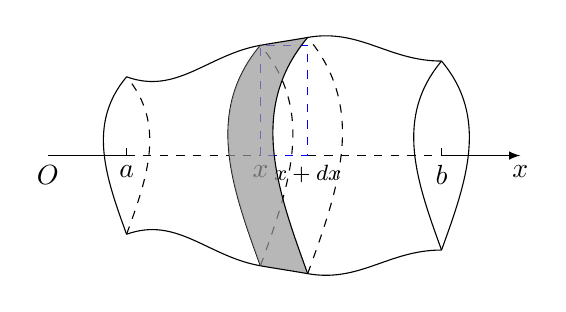
\begin{tikzpicture}[scale=1]
  % \draw [help lines] (0,-3) grid (6,3);

  \draw (0,0) -- (1,0);
  \draw[dashed] (1,0) -- (2.7,0);
  \draw[dashed] (3.3,0) -- (5,0);
  \draw[-latex] (5,0) -- (6,0);
  \node[below] at (0,0) {$O$};
  \node[below] at (1,0) {$a$};
  \draw (1,0) -- (1,0.1);
  \node[below] at (6,0) {$x$};
  \node[below] at (5,0) {$b$};
  \draw (5,0) -- (5,0.1);
  \node[below] at (2.7,0) {$x$};
  \node[below] at (3.3,0) {\footnotesize $x+dx$};
  \draw[dashed,blue] (2.7,0) -- (2.7,1.4) -- (3.3,1.4) -- (3.3,0) -- (2.7,0);

  % 左边
  \draw (1,-1) to [out=110,in=230] (1,1);
  \draw[dashed] (1,-1) to [out=70,in=-50] (1,1);

  % 左边的边框
  \draw (1,1) to [out=-20,in=190] (2.7,1.4);
  \draw (1,-1) to [out=20,in=170] (2.7,-1.4);

  % 中间 1
  \draw (2.7,-1.4) to [out=110,in=230] (2.7,1.4);
  \draw[dashed] (2.7,-1.4) to [out=70,in=-50] (2.7,1.4);

  % 阴影
  \begin{scope}
    \pgfsetfillopacity{0.7}
    \path[fill=black!40] (2.7,-1.4) to [out=110,in=230] (2.7,1.4) to [out=10,in=190] (3.3,1.5) to [out=230,in=110] (3.3,-1.5) to [out=170,in=-10] (2.7,-1.4);
  \end{scope}

  % 中间的边框
  \draw (2.7,1.4) to [out=10,in=190] (3.3,1.5);
  \draw (2.7,-1.4) to [out=-10,in=170] (3.3,-1.5);

  % 中间 2
  \draw (3.3,-1.5) to [out=110,in=230] (3.3,1.5);
  \draw[dashed] (3.3,-1.5) to [out=70,in=-50] (3.3,1.5);

  % 右边的边框
  \draw (3.3,1.5) to [out=10,in=180] (5,1.2);
  \draw (3.3,-1.5) to [out=-10,in=180] (5,-1.2);

  % 右边
  \draw (5,-1.2) to [out=110,in=230] (5,1.2);
  \draw (5,-1.2) to [out=70,in=-50] (5,1.2);
\end{tikzpicture}
